%!TEX root=main.tex

A heurística 1.2 surgiu como na tentava de melhorar a heurística 1. Esta heurística faz o que a sua predecessora já fazia e adicionalmente mais algumas avaliações semelhantes que visão evitar jogadas fatalistas ou aproveitar oportunidades ofensivas. Para tal a heurística considera além do \emph{número de possibilidades} o \emph{número de possibilidades fortes}. 
Para explicar o que o algoritmo entende como possibilidades fortes vamos atentar a segunda linha horizontal do tabuleiro do Pentago. 

\begin{table}[H]
\centering
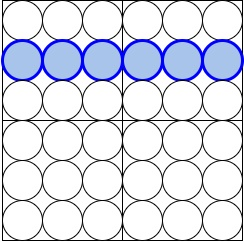
\includegraphics[height=3.5cm]{images/h12_hline.jpg}
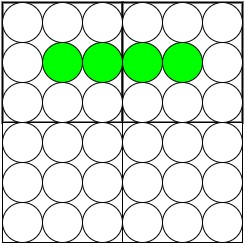
\includegraphics[height=3.5cm]{images/h12_fatal.jpg}
\end{table}

Podemos observar que o tipo de padrão usado na figura à direita é interessante do ponto de vista ofensivo, pois cria uma vitória garantida, e é contra este género de situações que o algoritmo tenta precaver-se ou tirar proveito ofensivo.
Para tal, o algoritmo contabiliza 2 tipos de casos. Denominemos esses tipos de tipo \emph{forte} e de tipo \emph{muito forte} sendo que qualquer caso que seja do tipo muito forte é também um caso do tipo forte mas o inverso pode não ser verdade. Considera-se um caso forte quando um grupo, dos definidos na heurística 1, está ocupado por peças de um jogador. Um caso muito forte acontece quando um grupo está ocupado por peças de um jogador e a sua extensão no mesmo quadrante se encontra sem uma peça adversária (podendo estar vazia ou não). Assim as 3 imagens seguintes ilustram respetivamente 2 jogadas do tipo muito forte e uma do tipo forte.

\begin{table}[H]
\centering
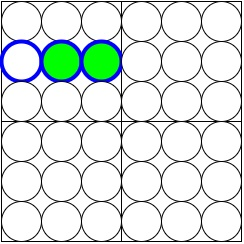
\includegraphics[height=3.5cm]{images/h12_VS.jpg}
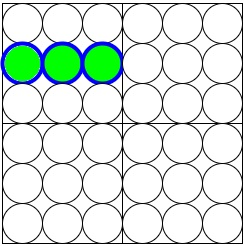
\includegraphics[height=3.5cm]{images/h12_VS2.jpg}
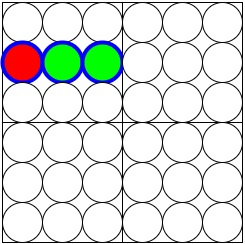
\includegraphics[height=3.5cm]{images/h12_S.jpg}
\end{table}

Depois de contabilizadas estes casos o número de jogadas fortes para a segunda linha horizontal é dada pela seguinte fórmula:
\begin{equation}
F_{hor2} = max( min(F_1,M_2) , min(M_1,F_2) )
\end{equation}
Onde $Fi$ e $Mi$ representam respetivamente o número de casos fortes e o número de casos muito fortes no quadrante $i$. Os quadrantes usados, são os que contêm a linha como mostra a figura seguinte.

\begin{table}[H]
\centering
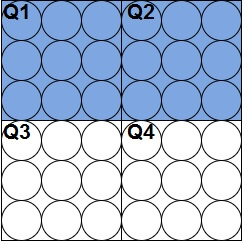
\includegraphics[height=3.5cm]{images/boardsQuadrants.jpg}
\end{table}

Assim, para melhor ilustrar a contabilização referida, são apresentadas abaixo exemplos onde o número de jogadas fortes para a segunda linha horizontal são respetivamente 1, 1, 1 e 2.

\begin{table}[H]
\centering
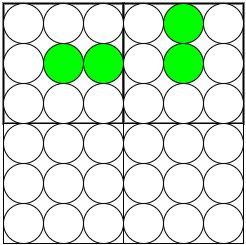
\includegraphics[height=4cm]{images/h12_ex1.jpg}
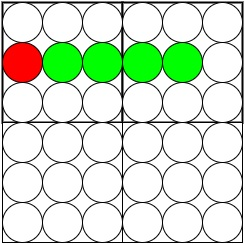
\includegraphics[height=4cm]{images/h12_ex2.jpg}
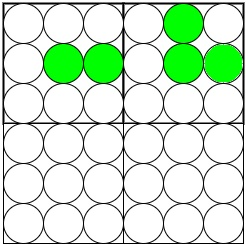
\includegraphics[height=4cm]{images/h12_ex3.jpg}
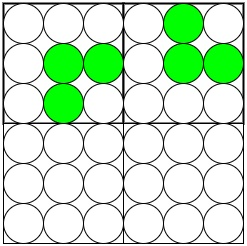
\includegraphics[height=4cm]{images/h12_ex4.jpg}
\end{table}

A mesmos cálculos são efetuados para as outras linhas (excluindo s diagonais menores que são tratadas de forma diferente) para ambos os jogadores. A heurística usa o número de jogadas fortes para o jogador (com valor positivo), para adversário (com valor negativo) e também as possibilidades da heurísticas 1. Todas estas componentes têm um peso associado que confere à heurística alguma flexibilidade podendo esta variar não só entre uma abordagem otimista ou pessimista mas também por abordagem mais passiva ou reativa.

Apesar destas considerações a heurística têm algumas dificuldades em lidar com  limitações de profundidade no Minmax pelo que foi implantada uma versão relaxada. Na sua versão relaxada consideram-se como fortes os blocos ocupados com pelo menos uma peça do jogador e nenhuma do adversário, tal como apresentado na ilustração abaixo.

\begin{table}[H]
\centering
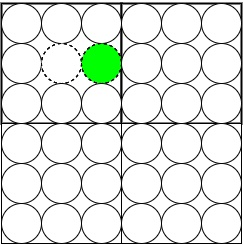
\includegraphics[height=4cm]{images/h12_relax.jpg}
\end{table}

Apesar de melhorar a sua predecessora também herda as suas fraquezas não sabendo lidar com as rotações do jogador adversário.

